\documentclass{beamer}
\usepackage[slovene]{babel}

\usetheme{Darmstadt}
\usecolortheme{dolphin}

\title{Predstavitev 1. domače naloge}
\author[G. Stanovnik]{Gal Stanovnik}
\institute{Univerza v Ljubljani, Fakulteta za strojništvo}
\date{\today}
\logo{

\includegraphics[width=1.8cm]{ul-fakulteta-za-strojnistvo}
}

\AtBeginSection[]
{
\begin{frame}
\frametitle{Kazalo}
\tableofcontents[currentsection]
\end{frame}
}


\begin{document}

\frame{\titlepage}

\section{Funkcijska datoteka}

\begin{frame}
\begin{block}{}
\frametitle{Funkcijska datoteka}
Najprej ustvarimo funkcijsko datoteko mcc\textunderscore pi in v njej definiramo funkcijo, ki kot rezultat vrne dve matriki z koordinatami naključno generiranih točk. V prvi matriki so točke, ki ležijo znotraj kroga, v drugi pa točke, ki ležijo izven kroga.
$a_{\text{x}}$ is different from $a_x$
\end{block}
\pause
\begin{block}{}
Če funkcijo pokličemo res dobimo dve matriki:
\end{block}
\end{frame}

\begin{frame}
\begin{figure}
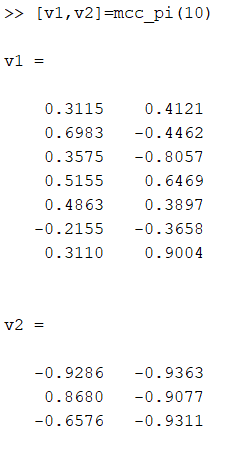
\includegraphics[height=220px]{Slika_matrik.png}
\end{figure}
\end{frame}

\section{Programska datoteka}

\begin{frame}
\begin{block}{}
\frametitle{Programska datoteka}
Najprej ustvarimo programsko datoteko calc\textunderscore pi. Ker nas zanima vpliv števila generiranih točk na točnost dobljenega približka števila $\pi$, lahko s for zanko izračunamo približek pri različnem številu točk:
\begin{figure}
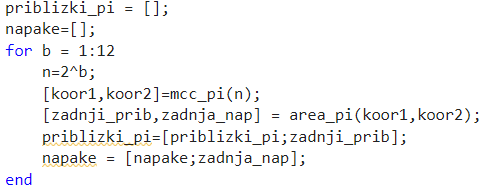
\includegraphics[height=80px]{For zanka.png}
\end{figure}
\end{block}
\pause
\begin{block}{}
Pri tem smo klicali funkcijo area\textunderscore pi, ki izračuna približek in napako približka. Definirali smo jo čisto na dnu programske datoteke.  
\end{block}
\end{frame}

\section{Anonimna funkcija}

\begin{frame}{}
\frametitle{Anonimna funkcija}
\begin{block}{}
Definirali smo anonimno funkcijo, ki prejme radij željene krožnice in vektor točk x. Vrne matriko vrednosti, v prvem stolpcu so vrednosti za pozitivne y koordinate, v drugi vrstici pa so vrednosti negativnih y-ov.
\begin{figure}
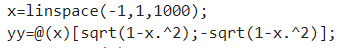
\includegraphics[width=0.6\textwidth]{Anonimna_funkcija.png}
\end{figure}
\end{block}
\end{frame}

\section{Vizualizacija}

\begin{frame}
\frametitle{Vizualizacija}
\begin{block}{}
Na en graf izrižemo točke krožnice, točke zunaj in točke znotraj kroga.
\end{block}
\begin{figure}
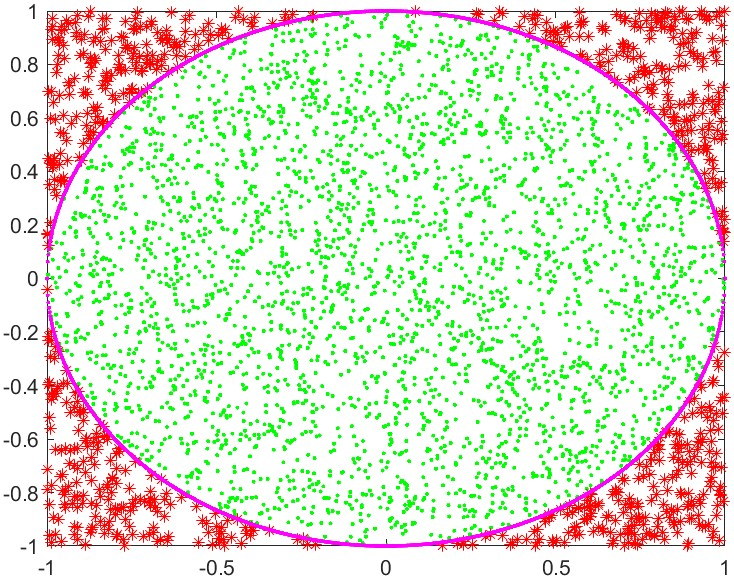
\includegraphics[height=120px]{Graf_1.0.jpg}
\caption{Točke izven krožnice so obarvane rdeče, točke znotraj pa zeleno. Točke na krožnici so vijolične.}
\end{figure}
\end{frame}

\end{document}